\graphicspath{{images/}}

\section{\thesection~Introduction}
\label{sec:introduction}

% Expand motivation, describe QFA, discuss alternative approaches.

% Dummy \citet{Lawless2010} citations \citep{Heydari2016} \citep{Addinall2008}.

% The bacteria \textit{Eschericia Coli} and yeast \textit{Saccharomyces
%   cerevisae} are unicellular organisms studied as a model prokaryote
% and eukaryote respectively. They grow in colonies, where cells may (be
% clones originating from a single cell or) belong to different genetic
% strains originating from different individual cells. In favourable
% conditions, growth is exponential and this makes growth rate a major
% component of fitness; faster growing strains quickly come to dominate
% the population. Growth rate is measurable and is often used to
% determine the fitness of microbial organisms. For unicellular
% organisms, growth rate is equal to cell cycle progression
% rate. Evolutionary pressure has led to rapidly dividing organisms with
% a compact genome of essential genes. These genes have been conserved
% in other species over billions of years of evolution. The eukaryote
% \textit{S. cerevisae}, is particularly useful for the study of other
% eukaryotes such as humans.


The bacteria \textit{Eschericia Coli} and yeast \textit{Saccharomyces
  cerevisae} are unicellular organisms studied as a model prokaryote
and eukaryote respectively. They grow in colonies, where cells may (be
clones originating from a single cell or) belong to different genetic
strains originating from different individual cells. In favourable
conditions, growth is exponential and this makes growth rate a major
component of fitness; faster growing strains quickly come to dominate
the population. At a certain point growth becomes limited and a
stationary phase is reached. For unicellular organisms, growth rate is
equal to cell cycle progression rate. Evolutionary pressure has led to
rapidly dividing organisms (such as \textit{E. Coli} and \textit{S.
  cerevisae}) with compact genomes of essential genes. These genes
have been conserved in other species over billions of years of
evolution. The eukaryote \textit{S. cerevisae}, is particularly useful
for the study of other eukaryotes such as humans.

The growth rate of microbial organisms is measurable and is often used
to determine fitness. In experiments, cell cultures are commonly grown
in two types of medium. In spot tests (phenotypic array), cultures are
pinned or inoculated on the surface of a solid agar containing
nutrients. In liquid culture assays, cultures are mixed in a liquid
medium containing nutrients. In both cases cultures are incubated and
growth is observed. Identical strains can grow differently between the
two mediums and disagreement in fitness estimates is currently an
issue \citet{Baryshnikova2010} (I couldn't find a paper specifically
talking about this issue but they have a correlation plot Fig2a where
correlations are worse with a liquid culture study by Jasnos and
Korona; in fact the Baryshnikova paper Fig3c seems to say that they
had strong correlation in their ``high-resolution liquid growth
profiling study''). I do not focus on this issue and exclusively study
fitness screens using solid agar.

% Where do cells grow surfaces films.

%%% Genetic interaction, SGA and QFA %%%

% Synthetic Genetic Array (SGA) and Quantitative Fitness Analysis (QFA)
% are high-throughput methods for obtaining quantitative fitness
% estimates of microbial cultures grown on solid agar
% \citep{Baryshnikova2010sga,Banks2012}.

% Fitness estimates can be used to infer genetic interaction or drug
% response and high-throughput methods allow this to be done on a
% genome-wide scale (see e.g. \citet{Costanzo2010}). In a typical
% genetic interaction study, a strain is made with a mutation in a query
% gene. Double mutants are created by introducing a second deletion in
% this strain. Typically one query gene is used per plate with
% replicates of many different deletions. By comparing the growth of
% double mutants with a control containing a neutral deletion, genetic
% interactions can be inferred. If a strain is fitter than the control
% then the deletion is said to suppress the defect of the query gene. If
% a strain is fitter than the control then the deletion is said to
% enhance the defect of the query gene. Either scenario suggests that
% the two genes interact and have a related function. Typically one
% query gene is used per plate and many replicates of each deletion are
% contained on each plate. Many plates can be analysed in
% high-throughput to explore whole genomes.


Fitness estimates can be used to infer genetic interaction or drug
response and high-throughput methods allow this to be conducted on a
genome-wide scale (see e.g. \citet{Costanzo2010,Andrew2013}). In a
typical genetic interaction screen, a strain is made with a mutation
in a query gene. Double mutants are created by introducing a second
deletion in this strain. By comparing the growth of double mutants
with a control containing a neutral deletion, genetic interactions can
be inferred. If a strain is fitter than the control then the deletion
is said to suppress the defect of the query gene. If a strain is less
fit than the control then the deletion is said to enhance the defect
of the query gene. Either scenario suggests that the two genes
interact and have a related function. Due to redundancy, single
deletions are often non-lethal. (Remove: Knock downs and conditional
mutations can also be used.) This allowed \citet{Costanzo2010} to
explore \(\sim\)75\% of the \textit{S. cerevisae} genome.


Synthetic Genetic Array (SGA) and Quantitative Fitness Analysis (QFA)
are high-throughput methods for obtaining quantitative fitness
estimates of microbial cultures grown on solid agar
\citep{Baryshnikova2010sga,Banks2012}. Typically one query gene and
replicates of deletion are contained in a rectangular array on a solid
agar plate. Many plates with different query genes and deletions can
be grown in high-throughput to explore whole genomes. I study data
from QFA which refers to quantitative estimation of fitness by
measurement and fitting of growth curves.


In a typical QFA procedure liquid cultures are incolulated onto solid
agar (containing nutrients (already mentioned above)) often with 384
cultures in 16x24 rectangular array. Initial inoculum density can be
varied to capture more or less of the growth curve. Dilute cultures
are inoculated with \(\sim\)100 starting cells
\citep{Addinall2011}. Plates are grown in incubation. Photographs of
whole plates are taken at timepoints throughout growth which typically
covers several days and captures the exponential and stationary growth
phases. Photographs are processed by Colonyzer \citep{Lawless2010} to
produce cell density estimates from the optical density of
cultures. Past analysis independently fit the logistic model, which
describes self-limiting growth, to the timecourse of each culture and
quantitative fitness estimates are defined in terms of the growth
constant, \(r\), and carrying capacity, \(K\). In contrast, SGA
typically uses an array of 1536 pinned cultures and an endpoint assay
of culture area (a single measurement) to quantify growth. The the
differential form and solution of the logistic model
\citep{Verhulst1845} (probably don't need this reference) are given in
Equations~\ref{eq:logistic_model}, where \(C\) represents cell density
and \(C_0\) is cell density at time zero.
% Logistic model equations
\begin{subequations}
  \label{eq:logistic_model}
  \begin{align}
    &\dot{C} = rC\left(1 - \frac{C}{K}\right)\\
    &C(t) = \frac{KC_{0}e^{rt}}{K + C_{0}(e^{rt}-1)}
  \end{align}
\end{subequations}
%
Fitting the logistic model to QFA data requires plate level or culture
level parameters for \(C_{t_{0}}\) and culture level parameters for \(r\)
and \(K\) making 769 or 1152 parameters per plate of 384 cultures.

//Could remove and just discus MDR when I get to the results//
The growth constant \(r\) could be used as a fitness measure. However,
\citet{Addinall2011} define a more complicated fitness measure as the
product of Maximum Doubling Rate (MDR) and Maximum Doubling Potential
(MDP) which they derive from logistic model parameters. MDR measures
the doubling rate at the beginning of the exponential growth phase,
when growth is fastest, and MDP is the number of divisions which a
culture undergoes from inoculation to the stationary phase.
%
\begin{subequations}
  \label{eq:MDR_MDP}
    \begin{align}
      MDR &= \frac{r}{log\left(\frac{2(K-C_0)}{K-2C_0}\right)}\\
      MDP &= \frac{log\left(\frac{K}{C_0}\right)}{log(2)}
    \end{align}
\end{subequations}
%
To improve the quality of fits QFA now uses the generalised logistic
model which requires an extra shape parameter for each culture to try
to improve the quality of fits to data. Standard and generalised
logistic model \(r\) are not equivalent so comparison relies on MDR
and MDP as fitness measures. The analysis of QFA data using both
models is available through the QFA R package \citep{qfa2016}.
//Could remove and just discus MDR when I get to the results//


//Could remove//
\citet{Addinall2011} used QFA and \textit{S. cerevisae} to screen for
genes involved in telomere stability which is related to ageing and
cancer and has implications for human health and disease. Hits from
this study have been successfully followed to discover new biology
\citep{Holstein20141259}. (To be honest I have no idea what they found
in that paper. Maybe I should leave this to biologist and out of my
report? We had a more general focus. Obviously I will mention the
Addinall paper when I describe p15 in the methods.)
//Could remove//
% Example use of QFA by Addinall \citep{Addinall2011} telomeres.
% And follow up Holstein and Clark \citep{Holstein20141259}




The solution to the logistic model is a sigmoidal curve. Growth begins
exponentially with rate \(rC\) and curtails as the population size
increases and cells begin to compete for space and nutrients or
interact in some other way. Cell density reaches a final carrying
capacity \(K\) at the stationary phase. In QFA, nutrients must diffuse
through agar to reach cells growing on the surface. It is plausible
that the carrying capacity \(K\) represents the point at which
nutrients either run out or growth becomes limited by the diffusion of
nutrients and is approximately stationary.

Since QFA aims to determine differences in the fitness of microbial
strains from measurements of differences in growth, fast and slow
growing cultures are often grown
side-by-side. Figure~\ref{fig:p15_section} shows a section of a QFA
plate from a study by \citeauthor*{Addinall2011} where this is the
case. (Cultures were inoculated with approximately equal cell density
but have grown at different rates to visibly different sizes after
\(\sim\)2.5 days.) It is likely that nutrients diffuse along gradients
between fast and slow growing neighbours causing growth to appear
faster or slower than would occur if it were independent. Further
support for such an effect comes from the experiment shown in
Figure~\ref{fig:stripes_images} where the same cultures are grown in
alternate columns on two separate plates but with cultures added or
removed from the neighbouring columns in between. Cultures in
Figure~\ref{fig:stripes_images}a), where neighbours were removed, grew
faster and larger than the same cultures in
Figure~\ref{fig:stripes_images}b), where neighbours were
added. Despite this, current QFA analysis using the logistic model
assumes that cultures grow independently and ignores possible
competition effects between neighbours. The sigmoidal curve of the
logistic model poorly fits QFA data in many cases. I aim to fit a
network model of nutrient dependent growth and diffusion to QFA data
to try to correct for competition and increase the accuracy and
precision of fitness estimates.

\begin{Figure}
  \centering
  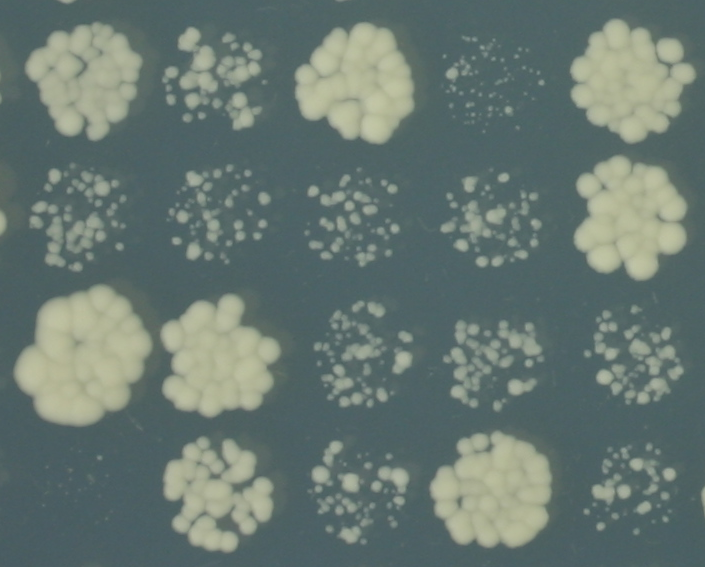
\includegraphics[width=\linewidth]{p15_section/p15_section}
  \captionof{figure}{\textbf{4x5 section of a QFA plate.} Taken from a
    16x24 format solid agar plate inoculated with dilute
    \textit{S. cerevisae} cultures.
  Image captured at \(\sim\)2.5d after inoculation and incubation at
  27\(^{\circ}C\).}
  \label{fig:p15_section}
\end{Figure}
\begin{Figure}
  \centering
  \includegraphics[width=\linewidth]{stripes/final/striped}
  \includegraphics[width=\linewidth]{stripes/final/filled}
  \captionof{figure}{\textbf{An experiment designed to examine
      competition.}\\
    A) QFA plate inocluated with a more concentrated
    \textit{S. Cerevisae} inoculum (no cells inocluated on alternative
    columns).\\
    B) Same as in A, but with strains of similar growth rate
    inoculated in the positions missing in A.}
  \label{fig:stripes_images}
\end{Figure}

Alternatively, competition effects could be dealt with experimentally
by randomising the location of cultures on repeated plates. This does
not require explicit knowledge or modelling of the source of
competition but reduces throughput, so, if possible, a modelling
approach is desirable. Poisoning of cultures by a signal molecule such
as ethanol, which \textit{S. cerevisae} produces in the metabolism of
sugars by fermentation, is another possible source of competition. QFA
does not measure nutrients or signal, so if more than one source of
competition exists, it will become very difficult to fit a model and
randomisation may be the best approach.  In an SGA study,
\citet{Baryshnikova2010} use statistical techniques to correct for
competition between fast and slow growing neighbours in end-point
assays of culture area. We hope that modelling the diffusion of
nutrients explicitly and using a full network diffusion model will
allow us to better correct for competition using fewer repeats. With
QFA, we can also use more information by fitting whole growth curves
rather than a single endpoint assay so a modelling approach offers to
be more powerful. Furthermore, modelling may help us to identify and
understand the source of competition. Simulation of an accurate model
will allow us to compare experimental designs and explore ways to
reduce competition effects.

//Diffusion Equation: I am probably going to have to reexplain this
when I get to the discussion so I could just leave until then.//
% Previous model of nutrient diffusion.
\citep{Reo2014} use a diffusion equation model to simulate nutrient
dependent growth of a single bacterial culture on a pertri dish in
two-dimensions. It would be too computationally intensive to fit a
similar model to a full QFA plate in three-dimensions, especially if
we are to use the model to process many plates from high-throughput
experiments. Therefore a simpler model of nutrient diffusion is
required.
//Diffusion Equation//


\textit{Lawless} (link blog) proposed a model of nutrient dependent
growth and competition using mass action kinetics and a network
diffusion model, hereinafter the competition model
(\ref{eq:reaction},\ref{eq:competition_model}). A schematic of the
model is drawn in Figure~\ref{fig:comp_model_schematic}. He represents
the nutrient dependent division of cells with the reaction equation,
\begin{subequations}
  \label{eq:reaction}
  \begin{align}
    &C + N \xrightarrow[]{b} 2C,
%    &rate = b_{i}[C][N],
  \end{align}
\end{subequations}
where \(C\) is a cell, \(N\) is the amount of nutrient required for
one cell division, and \(b\) is a rate constant for the reaction. The
identity of the limiting nutrient \(N\) is unknown but possible
candidates are sugar and nitrogen. He defines separate reactions
(\ref{eq:reaction}) with growth constant \(b_{i}\) for each culture,
indexed \(i\), on a plate and uses mass action kinetics to derive rate
equations for the amount of cells and nutrients associated with each
culture, \(C_{i}\) and \(N_{i}\). This gives the rate equation for
\(C_{i}\) (\ref{eq:competition_model}a) and the first term in the rate
equation for \(N_{i}\) (\ref{eq:competition_model}b). To arrive at the
full competition model, he models the diffusion of nutrients along
gradients between a culture \(i\) and its closest neighbours,
\(\delta_{i}\), by the second term in (\ref{eq:competition_model}b),
where \(k_{n}\) is a nutrient diffusion constant.
\begin{subequations}
  \label{eq:competition_model}
  \begin{align}
    % \frac{dC_{i}}{dt}& = b_{i}N_{i}C_{i},\\
    % \frac{dN_{i}}{dt}& = - b_{i}N_{i}C_{i} - k_{n}\sum_{j \epsilon \delta_i}(N_{i} - N_{j}).
    \dot{C_{i}}& = b_{i}N_{i}C_{i},\\
    \dot{N_{i}}& = - b_{i}N_{i}C_{i} - k_{n}\sum_{j \epsilon \delta_i}(N_{i} - N_{j}).
  \end{align}
\end{subequations}
Unlike the logistic model~(\ref{eq:logistic_model}), the competition
model has no analytical solution, and must instead be solved
numerically. If \(k_{n}\) is set to zero (in the independent limit),
the competition model reduces to the mass action equivalent of the
logistic model, hereinafter the mass-action logistic model (blog
ref)(, and has the same sigmoidal solution). (In this limit,
parameters of the competition model can be converted in terms of
parameters the logistic model (see methods section)).
%%%% could go to methods %%%%
When the competition model is fit to QFA data, \(C_{i}\) is observed
and \(N_{i}\) is hidden. Inoculum density, \(C_{t_{0}}\), is often
below detectable levels. By assuming that incolulum density is the
same for all cultures and that nutrients are distributed evenly
throughout the agar at time zero, plate level initial values of cells
and nutrients, \(C_{t_{0}}\) and \(N_{t_{0}}\) can be used. \(k_{n}\)
is assumed to be constant across the plate but must be inferred. There
is then a growth constant, \(b_{i}\), for each of 384 cultures on a
typical QFA plate making 387 parameters in total. The competition
model shares more information between cultures and has far fewer
parameters (387) than either the standard or generalised logistic
model which have 796 and 1153 total parameters respectively
\citep{Banks2012,qfa2016}.
%%%%%%%%%%%%%%%%%%%%%%%%%%%%%%
The competition model shares more information between cultures and has
fewer than half the parameters of either the standard or generalised
logistic model \citep{Banks2012,qfa2016}.





\begin{Figure}
  \centering
  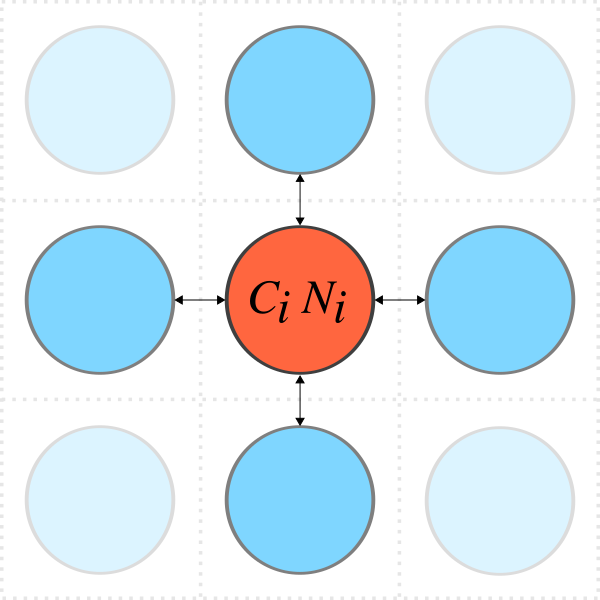
\includegraphics[width=\linewidth]{comp_model/comp_model_schematic}
  \captionof{figure}{\textbf{Schematic of the competition model.}
    Each circle represents a culture, indexed \(i\), growing in a
    rectangular array on the surface of a nutrient containing solid
    agar. Arrows represent a network of nutrient diffusion along
    gradients between cultures. \(C_{i}\) - amount of cells; \(N_{i}\)
    - amount of nutrients; \(k_{n}\) - plate level diffusion constant;
    darker blue circles \(\delta_{i}\) - closest neighbours of culture
    i.}
  \label{fig:comp_model_schematic}
\end{Figure}



% What is a nutrient?






\subsection{\thesubsection~Subsection}




%%% Local Variables:
%%% mode: latex
%%% TeX-master: "report"
%%% End:
